\ifCLASSOPTIONcompsoc
\IEEEraisesectionheading{\section{Introduction}\label{sec:introduction}}
\else
\section{Introduction}
\label{sec:introduction}
\fi


\IEEEPARstart{O}{nline} continual learning (OCL) is a special scenario of continual learning~\cite{wang2024comprehensive}. Taking the classification problem~\cite{liu2022model} as an example, OCL aims to develop a neural network that can accumulate knowledge of new classes without forgetting information learned from old classes. It is essential to note that the data stream encountered in OCL is non-stationary, with each sample being accessed only once during training. Currently, the main challenge of OCL is catastrophic forgetting (CF)~\cite{kong2023overcoming}, wherein the model experiences a significant decline in performance for old classes when learning new classes\cite{zhao2021memory}. 


The replay-based methods~\cite{lin2022anchor}, which replay a portion of previous samples, have shown superior performance for OCL~\cite{mai2022online}. In general, there are two ways to replay as shown in Fig.~\ref{fig:illustration}(a). The first is the proxy-based replay manner, which replays using a proxy-based loss function and softmax classifier. It calculates similarities between each anchor and the proxies belonging to all classes. Here, a proxy can be regarded as the representative of a class~\cite{yao2022pcl}, and the anchor represents a sample in a training batch. This manner is subjected to the ``bias'' issue resulting from class imbalance~\cite{lin2022anchor}. The second is the contrastive-based replay manner, which replays using a contrastive-based loss function and nearest class mean (NCM) classifier~\cite{mensink2013distance}. It computes similarities between each anchor and all samples in the same training batch. This manner is unstable and hard to converge during training. To sum up, these two manners have their corresponding shortcomings.  

\begin{figure*}[t]
\centering
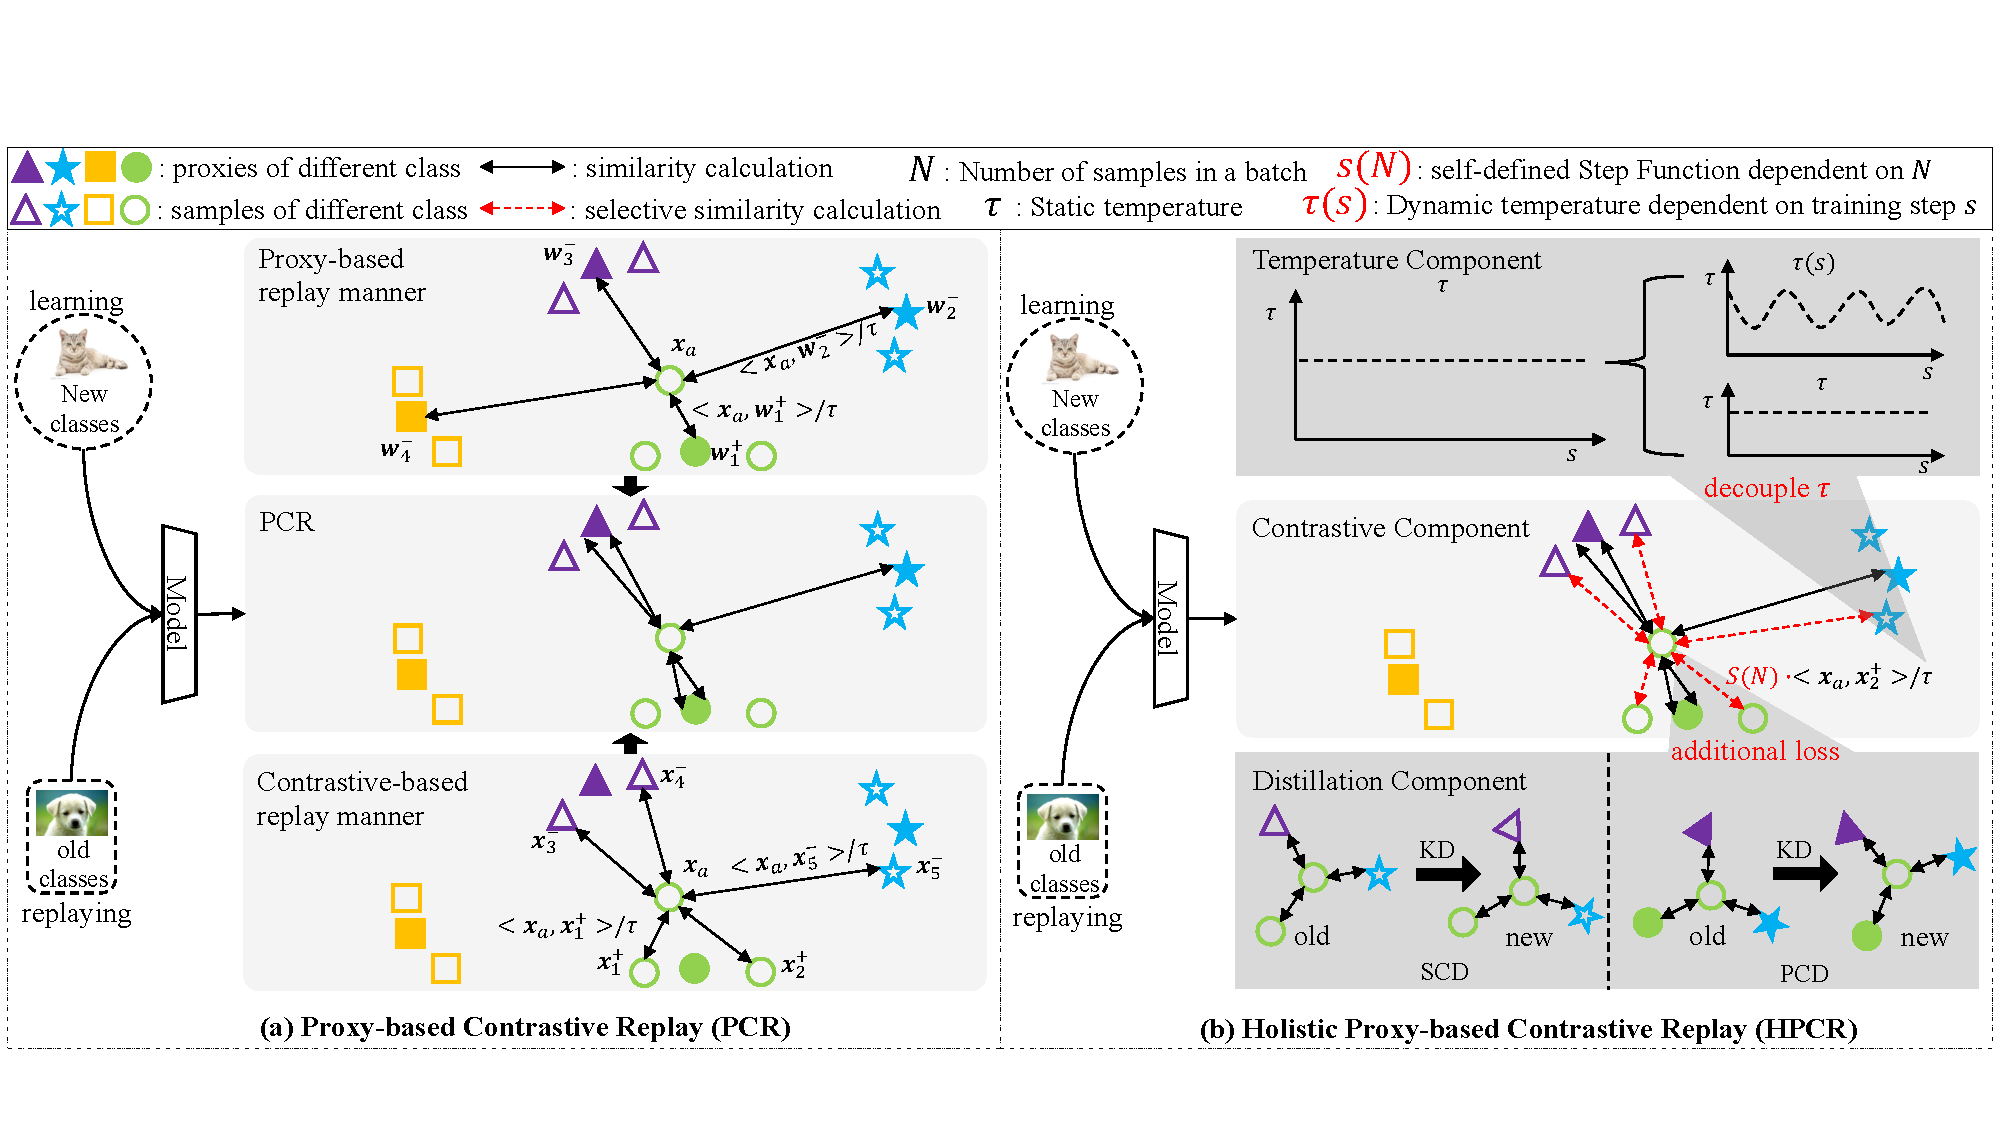
\includegraphics[scale=0.52]{sections/Figures/fig_illustration.pdf}
\vspace{-2ex}
\caption{Illustration of our work. (a) The example of existing replay manners. For each anchor sample $\bm{x}_a$, the proxy-based replay manner calculates similarities of all anchor-to-proxy pairs; the contrastive-based replay manner calculates similarities of all anchor-to-sample pairs in the same training batch; PCR only calculates similarities of selective anchor-to-proxy pairs in the same training batch. (b) The example of the proposed HPCR. The contrastive component conditionally produces anchor-to-sample pairs to PCR; the temperature component decouples the temperature coefficient into two parts based on their impacts on gradients and sets them differently; the distillation component constrains new anchor-to-sample pairs using the old ones (SCD), and distills old anchor-to-proxy pairs to the new ones (PCD).}
\label{fig:illustration}%
\vspace{-2ex}
\end{figure*}

\IEEEpubidadjcol

Our previous work~\cite{Lin_2023_CVPR} proposes proxy-based contrastive replay (PCR) method to handle these shortcomings. Specifically, we perform a comprehensive analysis and find that coupling both replay manners achieves complementary advantages. The proxy-based replay manner enables fast and reliable convergence with the help of proxies, thereby overcoming the problems of being unstable and hard to converge in the contrastive-based replay manner. Meanwhile, the contrastive-based replay manner can provide the proxy-based replay manner with a new way of selecting anchor-to-proxy pairs, which has been proven to effectively address the ``bias'' issue~\cite{ahn2021ss,caccia2021new}. With these inspirations, PCR calculates similarities between each anchor and the proxies whose associated classes of samples appear in the same batch as illustrated in Fig.~\ref{fig:illustration}(a). 

In this work, we conduct an in-depth analysis of PCR and explore its potential for improvement. Specifically, we derive the gradient propagation process of PCR in the classifier based on the one for general proxy-based loss. The gradient analysis shows that PCR benefits from the number of samples of different classes in each training batch, further confirming its effectiveness and reliability. However, our limitation analysis reveals that PCR still has shortcomings in three key areas: 1) PCR considers the relations between anchor-to-proxy pairs but ignores the relations between anchor-to-sample pairs. It results in insufficient \textbf{feature extraction capability} of the model, particularly in scenarios with large training batches where anchor-to-sample pairs contain important semantic information. 2) The simplistic setting of the temperature coefficient in PCR overlooks its impact on the gradient propagation process. This oversight undermines the model's \textbf{generalization capability}, as the use of a static constant fails to optimize effectively. 3) Old classes included in the learning process alongside new classes continue to encounter bias issues during training. It implies that there is still room for improvement in the model's \textbf{anti-forgetting capability}. Hence, PCR can be enhanced by overcoming these limitations.


To this end, we develop a more comprehensive method named holistic proxy-based contrastive replay (HPCR). As illustrated in Fig.~\ref{fig:illustration}(b), HPCR consists of three components. 1) The \textbf{contrastive component} incorporates anchor-to-sample pairs conditionally into PCR to improve the model's feature extraction capability, capturing more fine-grained semantic information when dealing with large training batches. Specifically, we introduce a step function $s(N)$ to regulate the importance of the anchor-to-sample pairs. When the number of samples is small, their contribution is set as 0; otherwise, it is 1. 2) Meanwhile, the \textbf{temperature component} decomposes the temperature coefficient into two parts based on their influence on gradients. One part is assigned a static constant value, while the other is denoted as a dynamic function value to strengthen the generalization capability, promoting the acquisition of novel knowledge. 3) Additionally, the \textbf{distillation component} imposes further constraints on the replaying process to enhance the anti-forgetting capability, preserving more historical knowledge. This component consists of two knowledge distillation (KD) mechanisms: proxy-based contrastive distillation (PCD) and sample-based contrastive distillation (SCD). The former distills the old anchor-to-proxy correlations into the new ones, while the latter constrains the new anchor-to-sample correlations based on the old ones. 

Our main contributions can be summarized as follows:
\begin{itemize}
\item[1)] We perform further analyses of the PCR. The gradient analysis verifies the effectiveness and reliability of PCR, while the limitation analysis suggests that PCR still has three limitations and can be further improved.

\item[2)] We develop a more holistic method based on PCR, named HPCR, which consists of a contrastive component, a temperature component, and a distillation component. These three components improve the model's feature extraction, generalization, and anti-forgetting capabilities, respectively.

\item[3)] We conduct extensive experiments on four datasets, and the empirical results consistently demonstrate the superiority of HPCR over various state-of-the-art methods. We also investigate and analyze the benefits of each component by ablation studies. And the codes are open-sourced at \url{https://github.com/FelixHuiweiLin/PCR}.
\end{itemize}

This work is an extension of our conference version presented in~\cite{Lin_2023_CVPR}. It offers a more comprehensive approach, which can be delineated into four aspects: (i) This version includes a gradient analysis of PCR, which enhances its theoretical foundation and helps us discover its limitations. (ii) This version conditionally integrates anchor-to-sample pairs into PCR to augment the model's feature extraction capability, treating it as a contrastive component. (iii) This version introduces a temperature component to enhance the model's generalization ability and a distillation component to improve the model's anti-forgetting capability. (iv) Furthermore, more experiments are conducted to explore the proposed method, which includes utilizing a new dataset (Split TinyImageNet), conducting additional ablation studies, and visualizations.